\documentclass[12pt, letterpaper]{article}

\usepackage{amsmath} %% Allows for mathematical expressions such as binomials.
\usepackage{color} %% Allows text to be typeset in color.
\usepackage{amssymb}

%% These allow Me to add Images to the Book.
\usepackage{graphicx}
\graphicspath{ {images/} }

%% Enables hyperlinks.
\usepackage{hyperref}


% Typeset Algorithms.
\usepackage[subsubsection]{algorithm}
\usepackage{algorithmic}

% Make the Captions small and italicized.
\usepackage[font={small,it}]{caption}


%% Makes BigO easier.
\newcommand{\bigO}{\mathcal{O}}
\newcommand{\bigOmega}{\Omega}
\newcommand{\bigTheta}{\Theta}

%% Redefines the varnothing symbol as the symbol for an empty set.
\let\emptyset\varnothing

%%
\oddsidemargin0cm
\evensidemargin0cm
\topmargin-2cm     % These lines increase the amount of usable space and save trees.
\textwidth16.5cm
\textheight23.5cm  

%%\setcounter{tocdepth}{4} %% set the table of contents detail depth.

%% Types of organizational sections.s
%%\part{}
%%\chapter{}
%%\section{}
%%\subsection{}
%%\subsubsection{}
%%\paragraph{}
%%\subparagraph{}

\begin{document}

\title{\color{blue}Extracting Curves from Subdivision Surfaces}
\author{Written by Bryce Summers \texttt(BryceSummers.com), Advised by Keenan Crane}
\date{\color{red}Last Updated: \today}
\maketitle

\newpage

\tableofcontents
\newpage

\section{Abstract}

	Effective communication of technical ideas often demands compelling mathematical diagrams and visualizations. 
	Just as TeX makes the best practices of professional mathematical typesetters accessible to everyday users,
	we aim to codify and automate best practices of professional mathematical illustrators.
	Currently, however, there is a functionality gap between 3D modeling software and 2D illustration software.
	The former allows users to manipulate 3D geometric information, while the latter allows users to manipulate aesthetic and stylistic information.
	In our work we wish to bridge the gap between these two types of software by extracting relevant curves from views of 3D Catmull-Clark subdivision 
		surfaces that visually communicate geometric relationships in the form of projected 2D Bezier curves amenable to traditional aesthetic design.


\newpage

\section{Introduction to the Problem}

	\subsection{Software Paradigms}

		Our work seeks to bridge a functionality gap between 3D Modelling software and 2D Illustration software. We will start out by describing each of these
		software paradigms and their strengths and weaknesses.

		\subsubsection{3D Modeling Software}

		Traditional 3D modeling software, such as the open source Blender program, are used primarily for creating defining the geometry and visual appearance of models to be 
		used in various applications such as 3D animation, the automative industry, and architectural visualization.
		These programs use the latest and greatest algorithms in the fields of computational geometry, rendering, and Computer Aided Design,
		but they do not have the capability to stylize their models with prescision. Many of them are geared towards rendering the models using 
		realistic models of light transport. As discussed in \cite{JDA08}, realisitic lighting is not necessarily the best stylistic descision for communicating
		geometric information about an object. Please see \ref{fig:photorealistic_rendering} for an example realistically rendered image.
		Please see \ref{fig:keenan_cow} for a typical 3D model as might be seen during manipulation in a 3D Modeling program. The visual style communicates
		the individual discrete vertices, edges, and faces that a user can modify which is important to a person constructing a 3D model, but it does not
		emphasize visual information that would be important to a geometer or a person seeking an traditionally aestetically enjoyable images.

		\begin{figure}[h]
		\centering
		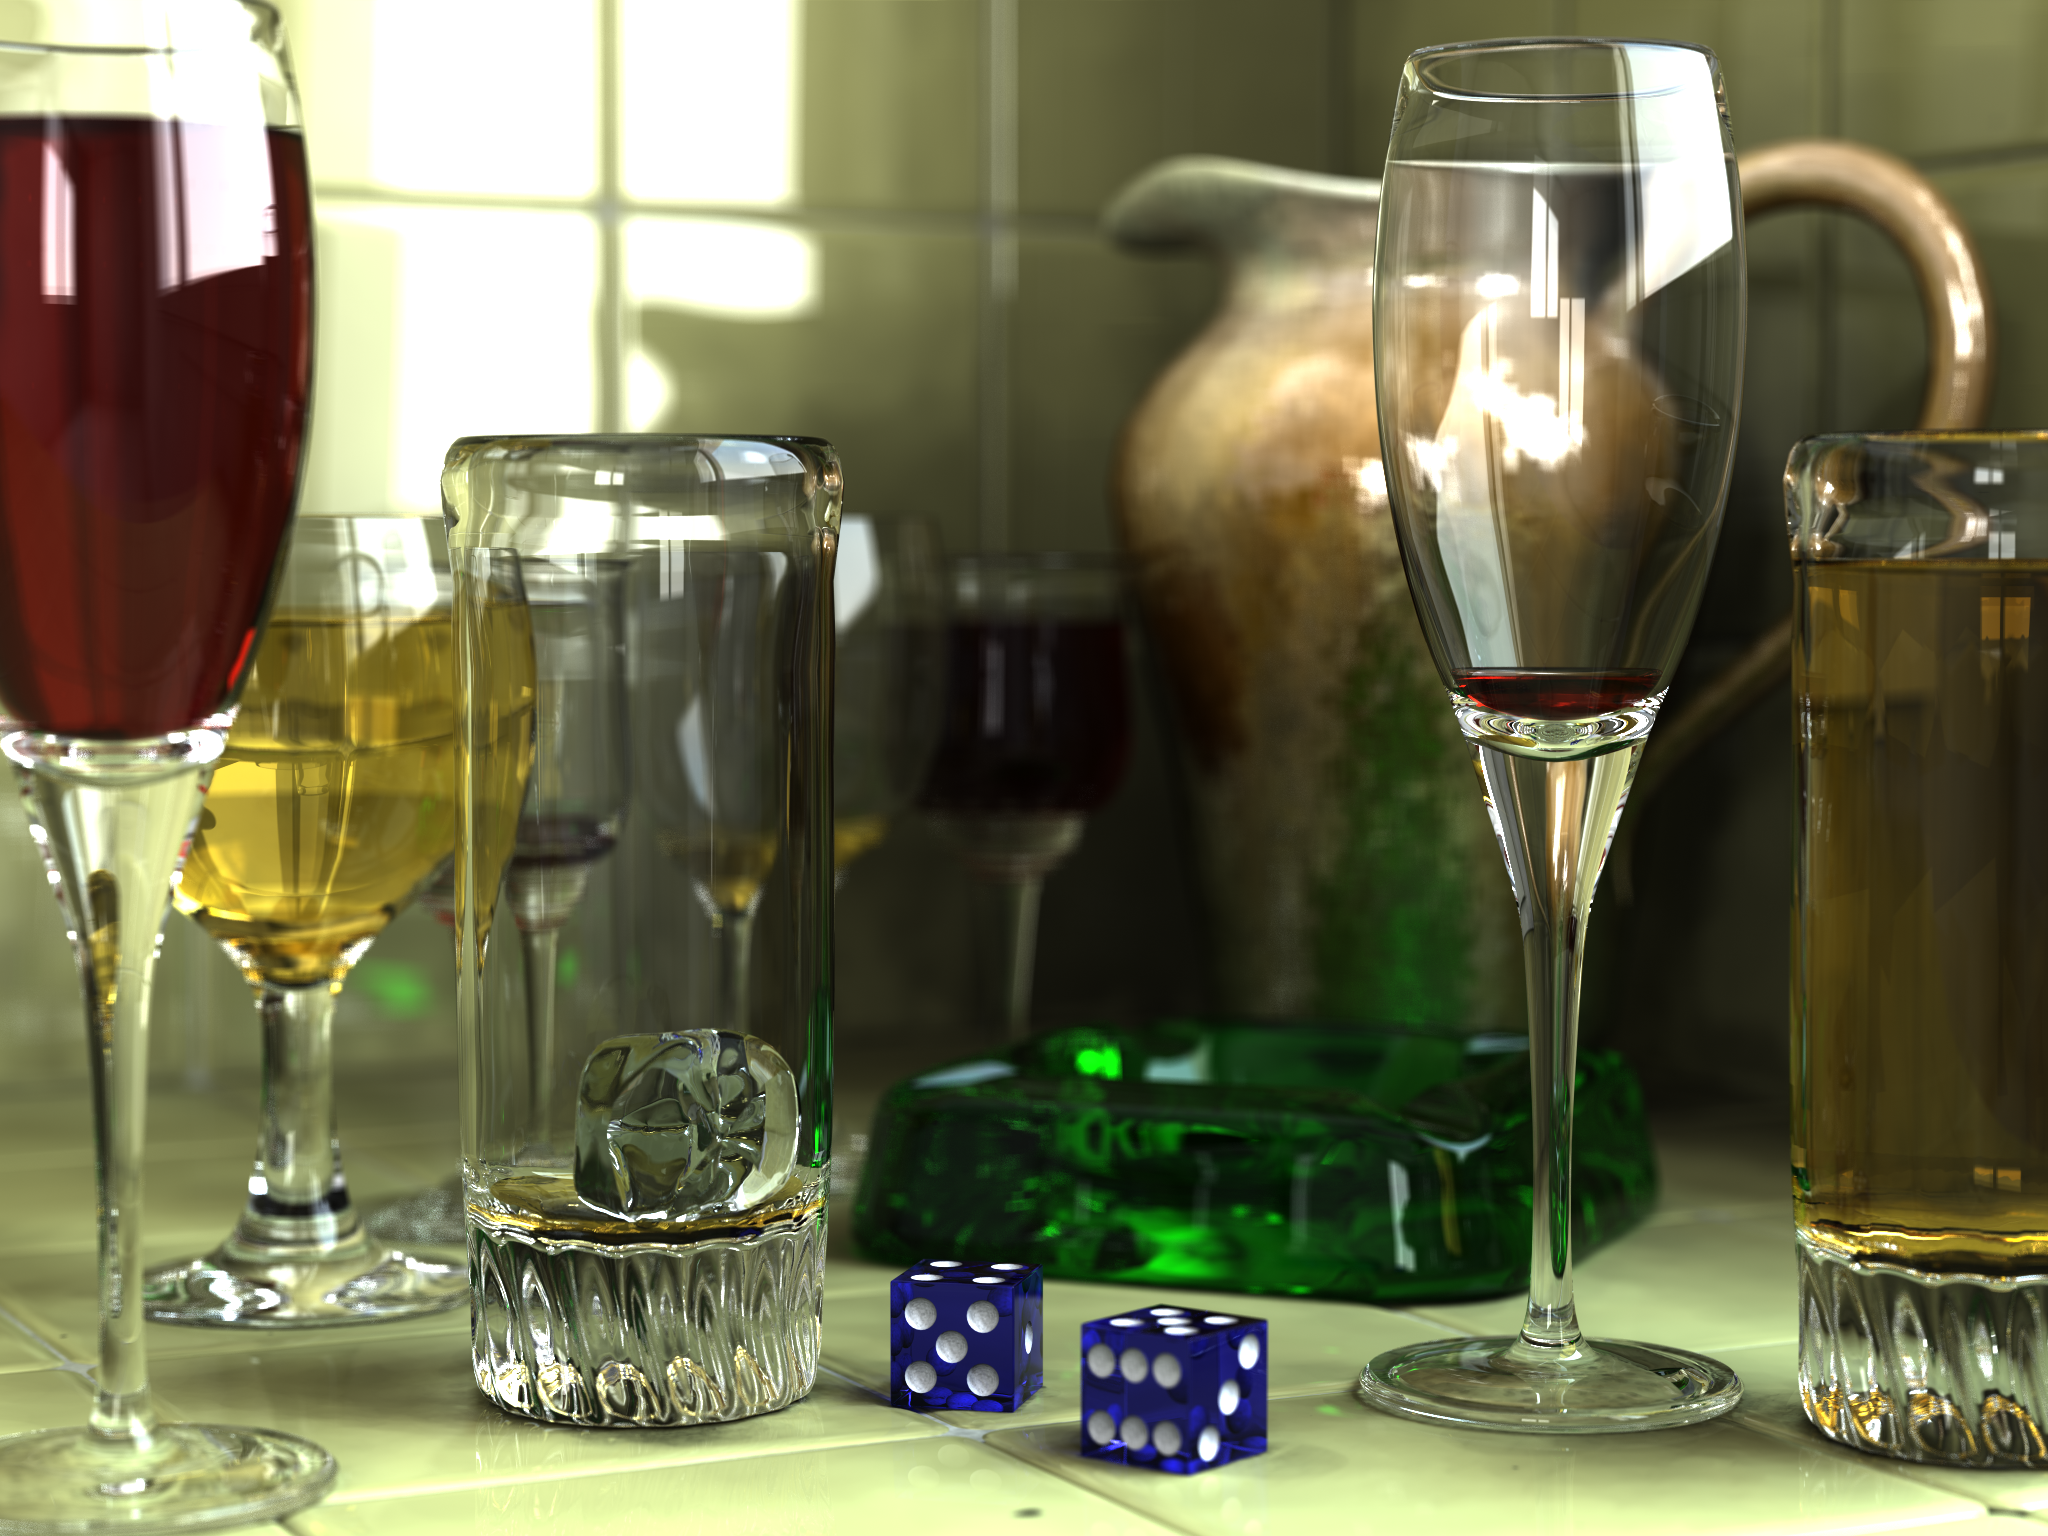
\includegraphics[width=0.5\textwidth]{PhotorealisticRendering}
		\caption{3D Modeling system are often used to produce photorealistic imagery, which is not always the proper best at communicating geometric information as discussed in \cite{JDA08}.
				Image Credit: Gilles Tran on Wikipedia.}
		\label{fig:photorealistic_rendering}
		\end{figure}

		\subsubsection{2D Illustration Software}

		2D illustration software, such as the open source Inkscape, are used primarily by designers and communicators to create 2D svg illustrations that
		communicate ideas, rather than realistic visual artifacts. They have a lot of capabilties for modifying the colors and stroke sizes of lines and interiors,
		labeling important features with textual boxes and arrows, and compositing different visual objects on top of each other through blending.
		While they are great at manipulating the aestetics of images, they do not necessarily understand 3D geometry and take it into account in the manipulations
		that they support. Please see Figure : \ref{fig:cornell_box_illustration}, which is an example 2D illustration that we created in Inkscape that communicates light transport within a traditional Cornell Box scene.

		\begin{figure}[h]
		\centering
		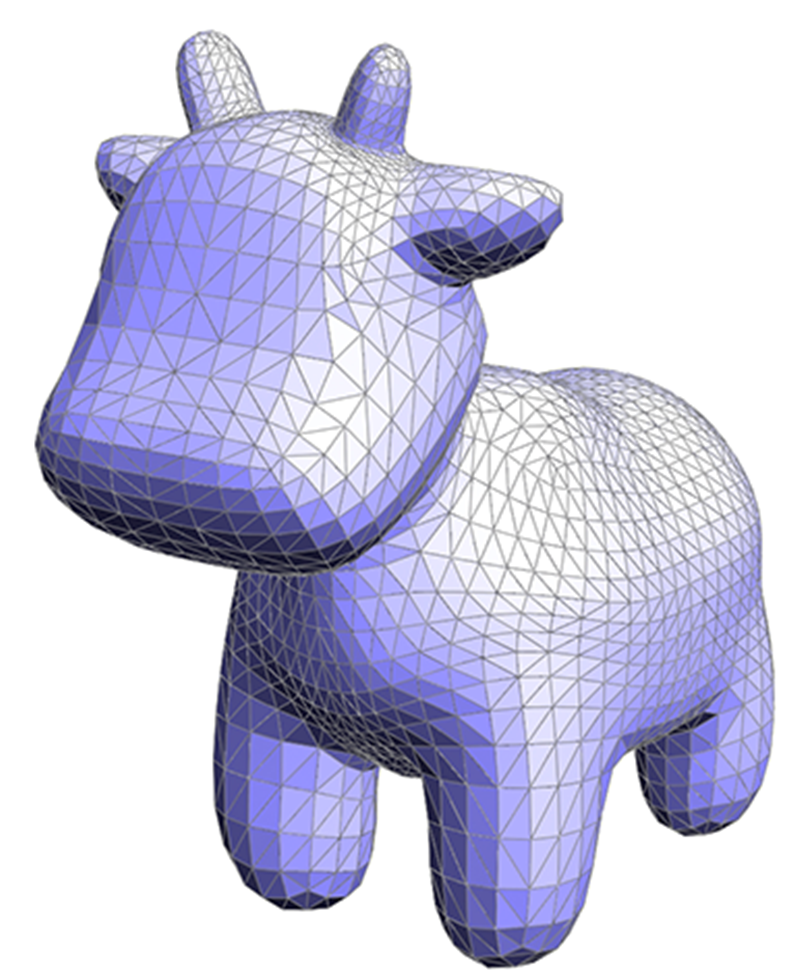
\includegraphics[width=0.5\textwidth]{KeenanCow}
		\caption{Typical 3D model that is manipulated in a 3D modeling program.}
		\label{fig:keenan_cow}
		\end{figure}

\newpage

\section{Background/Prior Work}

	\subsection{Important 2D curves for projected 3D models.}

		Various curves on surfaces communicate important geometric information. Here is a list of some relevant curves that folks have been
		trying to extract from surfaces in the past.

\begin{itemize}
	\item		Integral Lines: lines that follow the gradient of a function defined on a surface from one critical point to another. These may be used to form the Morse - Smale complex
			which segments the model into regions with similar monotonic functional behavior.
	\item		Parameterization curves are useful in showing lines along a collection of quadrilaterals and showing global coordinate systems.
	\item 	Silhouette curves communicate the visual extent of the model and the boundary.
	\item 	Minnimum - Maximum curvature lines communicate the curvature of the model and locally intuitive coordinate systems.
	\item        Geodesic curves communicate the path on the surface of minnimum distance between two points on a surface.
\end{itemize}

	\subsection{2D methods for extracting these curves}

		Many people have extracted silhouette curves by simply tracing the exterior boundary of a 2D rasterization of the surface. This approach suffers from 
		discretization and sampling problems and does not provide much information about the 3D geometric structure of the silhouette curves.
		For instance, they can't be used to compute direct shadows.
		It also may be possible to extract silhouette curves using an algorithm akin to the marching squares, but again it suffers from the same sorts of problems.
	
	\subsection{Catmull - Clark Subdivision Surfaces}
	
		Naively we could directly evaluate these curves over the linear patches defined on standard polyhedral 3D models,
		but much like the results found in \cite{Eisemann08},
		such lines would jitter back and forth over boundaries and would not converge to smooth natural and correct looking curves even after substantial
		subdivision of the surface. Please see Figure \ref{fig:Eisemann_linear_patches} for example of Eisemann et Al's attempt to extract silhouette
		curves from linear patches. We therefore wish to work on Catmull - Clark Subdivision surfaces that allow us to take a discrete quadrilateral control mesh
		and perform calculations on its limit defined subdivision surface, instead of any intermediate discrete representation.
		Please see Figure : \ref{fig:subDDef} for an illustration of control meshes and limit surfaces.

		\begin{figure}[h]
		\centering
		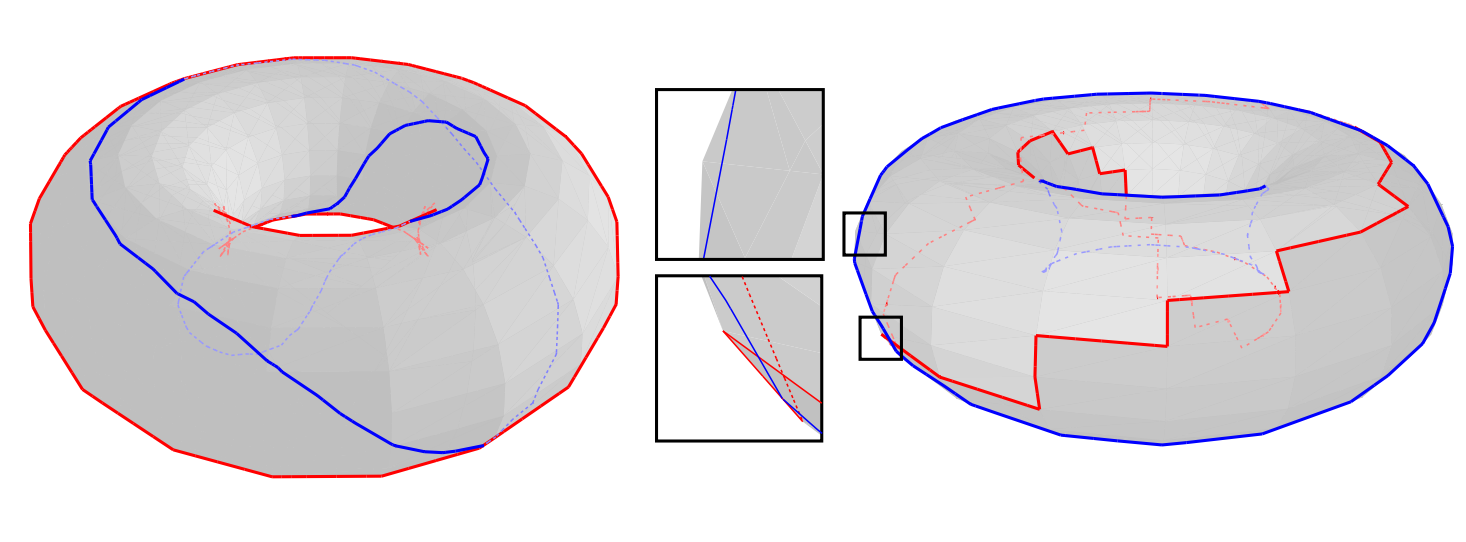
\includegraphics[width=0.5\textwidth]{Eisemann08_linear_patches}
		\caption{Linear Patches Silhouette curves either produce staircase patterns or don't properly lie on the geometry, even in the limit. Image Credit: \cite{Eisemann08}.}
		\label{fig:Eisemann_linear_patches}
		\end{figure}

		\begin{figure}[h]
		\centering
		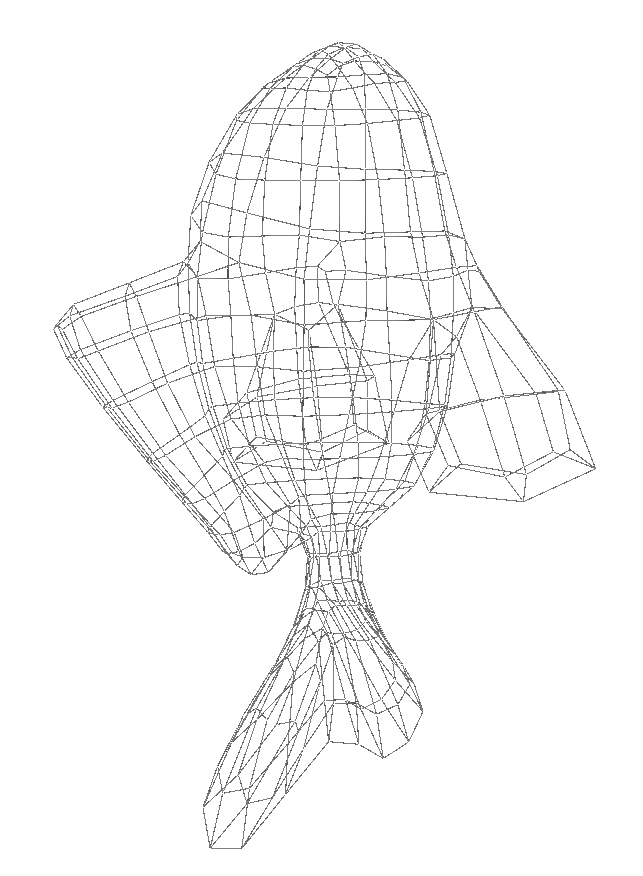
\includegraphics[width=0.3\textwidth]{fish_cm}
		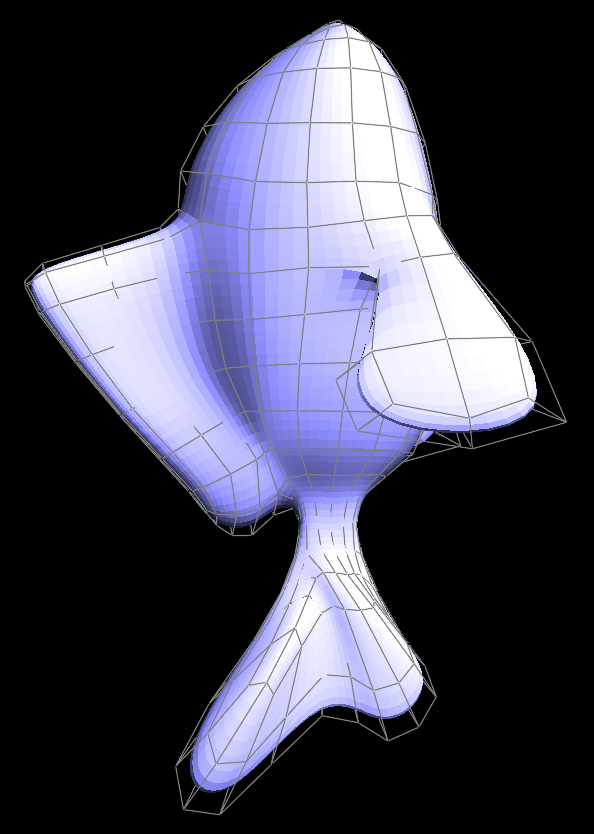
\includegraphics[width=0.3\textwidth]{fish_cm_and_patch}
		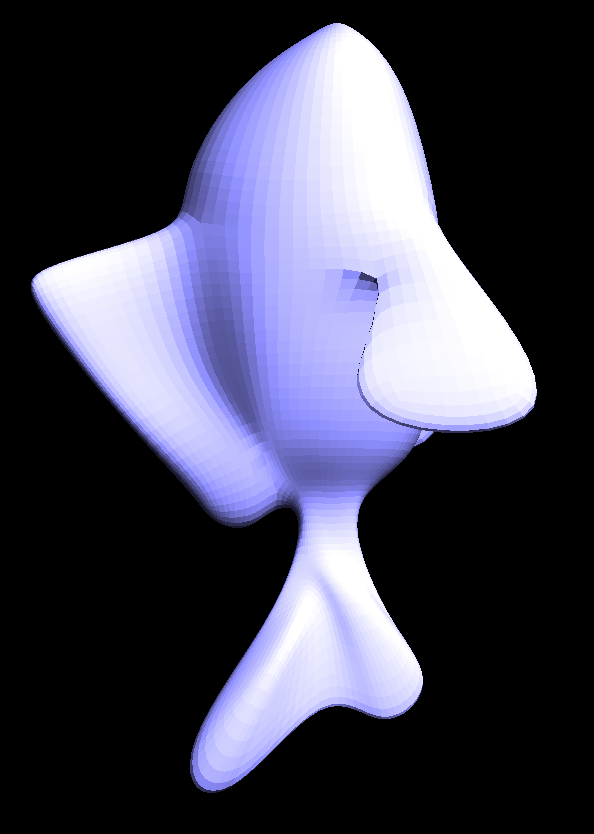
\includegraphics[width=0.275\textwidth]{fish_patch}
		\caption{A model of a fish represented from on the left by its control mesh and on the right by a geometry patch approximation of its Catmull-Clark limit surface. 
				Please note the discontinuity in shading at the top of the fish's back finn.
				This is caused by the vertices of degree 5 in that vicinity and is fixed by using tangent patches to interpolate the tangents across boundaries.}
		\label{fig:subDDef}
		\end{figure}

	\newpage

	\subsection{Loop - Shaeffer Approximations}
	
		No matter how finely we refine a traditional Catmull - Clark surface, it will still be a collection of linear patches which suffer from the same problems as 
		in \cite{Eisemann08}.  We therefore get around this problem by directly computing a continuous and differentiable approximation of the limit surface
		via the scheme described in \cite{Loop}
		We can create a one-to-one correspondence between faces in the control mesh and bicubic bezier surfaces (a.k.a "patches") that approximate the 
		limit Catmull - Clark subdivision surface that the faces represent.
		To do so, we follow the procedure outlined in \cite{Loop}.
		We therefore are able to derive control points for a geometry patch which we will denote $G_{ij}$ (Figure: \ref{fig:G}) and two tangent patches, 
		one for each principal parameter direction along the bicubic patch (Figure: \ref{fig:dU} and Figure: \ref{fig:dV}).
		The tangent patches are necessary, because the geometry patches only exhibit G0 continuity in the presense of extraordinary vertices.
		Since any quadrilateral mesh that is not homeomorphic to a torus must contain an extraordinary vertex,
		it is essential that we use the tangent patches to ensure effective differentiability everywhere along the surface formed by the union of the bicubic patches.
		
		For the remainder of the paper, we will be using these Loop - Schaeffer patch defined surfaces defined on quadrilateral meshes and refer to them simply as "Surfaces".



\section{Methodology}

	\subsection{Definitions of Calculus on Bicubic Patches}
	
	In this section we will discuss some fundamental calculus computations involving the patches that will be used in curve extraction algorithms.
	
		\subsubsection{Bezier Surfaces}
		The beauty of the bicubic patch approximations is that they allow us to transition from discrete math to well defined continuous math.
		
		The Bernstein Polynomials are defined as follows:
		
		$$\mathcal{B}_{i}^{n}(x) = \binom{n}{i}x^{i}(1-x)^{n-i} \; \textbf{for} \; i \in \{0, \cdots, n\}  $$
		
		Two-dimensional Bezier surfaces are defined parametrically as follows: 
		
		$$[0, 1] \times [0, 1] \rightarrow \mathbb{R}^{3} : \sum_{i=0}^{n}{\sum_{j=0}^{m}{\mathcal{B}_{i}^{n}(u) \mathcal{B}_{j}^{m}(v) C_{i, j}}}$$
		
		where $n, m$ is the degree of the surface, which is represented by $(n + 1) \cdot (m + 1)$ control points denoted genarically here by $C_{ij}$.
		
		The geometry patch surfaces are of degree (3, 3) and are therefore represented by the 16 control points $G_{ij}$ as follows:
		
		$$g(u, v) = \sum_{i=0}^{3}{\sum_{j=0}^{3}{\mathcal{B}_{i}^{3}(u) \mathcal{B}_{j}^{3}(v) G_{i, j}}}$$
		
		\subsubsection{Partials Defined by Geometry Patches}

		We can easily take partial derivatives of a Geometry Patch as follows:

		$$g_{u^{m}v^{n}} = \frac{\partial g}{\partial u^{m} \partial v^{n}} = \sum_{i=0}^{3}{\sum_{j=0}^{2}{\mathcal{B}_{i, 3}^{(m)}(u) \mathcal{B}_{j, 3}^{(n)}(v) G_{i, j}}}$$

		where $m$ is the degree of differentiation in $u$ and $n$ is the degree of differentiation in $v$.

		\subsubsection{Partials Defined by Tangent Patches}
		
		We can easily take partials of $g$ in $u$ and $v$ by differentiating the relevant $u$ or $v$ parameterized bezier function,
		but for the most part we will not make use of this pleasantry, because the geometry patches may be non differentiable on the boundaries.
		We will instead evaluate the partials from the tangent patches.
		
		$$g_{u} := \frac{\partial g}{\partial u} = \sum_{i=0}^{3}{\sum_{j=0}^{2}{\mathcal{B}_{i}^{3}(u) \mathcal{B}_{j}^{2}(v) U_{i, j}}}$$
		$$g_{v} := \frac{\partial g}{\partial v} = \sum_{i=0}^{2}{\sum_{j=0}^{3}{\mathcal{B}_{i}^{2}(u) \mathcal{B}_{j}^{3}(v) V_{i, j}}}$$

		\subsubsection{Normal}

		The normal direction is defined for any point on the surfaces as follows:

		$$N(u,v) = g_{u} \times g_{v} (u, v)$$

		\subsubsection{Visibility}

		Given a fixed yet arbitrary viewing direction $E$ we can define the visibility function as follows:

		$$f(u, v) = N(u, v) \cdot E$$

		A location $(u, v)$ in parameter space on a surface is visible if and only if $f(u, v)$ is negative.
		It is important to note that we are assuming an orthonormal fixed viewing direction, instead of a perspective projection,
		because it simplifies our mathematics. \ref{XJY98}

		\subsubsection{Silhouette Curves and Points}

		A Silhouette point $sp$ is any point such that the visibility function is zero. In other words the following must hold:
		$$sp = g(u, v) \textbf{ and } f(u, v) = 0$$

		A silhouette curve contains a closed ordered set of silhouette points. In other words they are defined as the boundary between the visible and non visible regions of the surface.

		\subsubsection{Gradient Descent}

		// FIXME : Mention the Armijo and Wolfe conditions.

	\subsection{Extracting Parameterization Curves}

		Extracting parameterization curves is quite straightforward. Start corner of a patch and then procceed in either the u or v direction as desired until you either get back to the original point or you encounter an extraordinary vertex.
		Please see a more formal description in Algoriithm: \ref{alg:TraceParameterizationCurves}, noting that the computation is symmetric for the u or v direction.
		Please see Figure: \ref{fig:parameter_aligned_curves_torus} for example of parameterization curves extracted from a torus.

		\begin{algorithm}                      % enter the algorithm environment
		\caption{Given a surface, a point, and a fixed yet arbitrary u direction, this procedure computes the visible and nonvisible portions of an axis algined parameter curve.}
		\label{alg:TraceParameterizationCurves}       % and a label for \ref{} commands later in the document
		\begin{algorithmic}                    % enter the algorithmic environment
			\REQUIRE The surface must be \textbf{continuous}, and implied by this document be made of quadrilaterals.
			\ENSURE Returns a set of visible and nonvisible portions of the parameter curve going through the input poin in the u direction.
			\STATE \textbf{begin}
			\STATE $S \Leftarrow $ Silhouette Point Finding Algorithm \ref{alg:FindSilhouettePoints}.
			\FOR{ Point $p \in S$}
			        \STATE $(u_{0}, v_{0}) \Leftarrow (p.u, p.v)$
				\STATE $(u, v) \Leftarrow (u_{0}, v_{0})$
				\REPEAT
				        \STATE $(dv, -du) \Leftarrow \nabla f(u,v)$
					\STATE normalize $(du, dv)$.
					\STATE $(u', v') \Leftarrow (u, v) + \epsilon \cdot (du, dv)$
					\IF{Line $(u, v) \Leftrightarrow (u', v')$ crosses a patch boundary}
						\STATE Remove the closest root on the boundary from $S$ to prevent duplicate tracings.
					\ENDIF
					\STATE $(u, v) \Leftarrow$ Gradient Descent on $c \cdot \nabla(f^{2}(u',v'))$, where $c$ is any positive number.
				\UNTIL{$(u, v) ~= (u_{0}, v_{0})$} \COMMENT{This should be checked within some $\epsilon$ dependant bounds.}
				\COMMENT{// FIXME: I should probably just have the algorithm terminate if we encounter the original root point on a boundary cross...}
			\ENDFOR
			\STATE \textbf{end}
		\end{algorithmic}
		\end{algorithm}

		\begin{figure}[h]
		\centering
		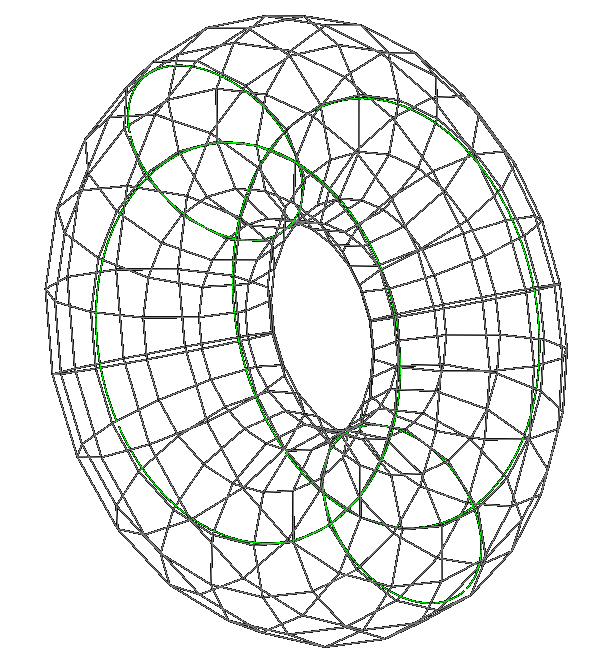
\includegraphics[width=0.5\textwidth]{Parameter_aligned_curves}
		\caption{Some Example Parameterization curves along the major axis of a torus. FIXME : Replace this with a better picture with thicker lines.}
		\label{fig:parameter_aligned_curves_torus}
		\end{figure}

	\subsection{Extracting Silhouette Curves}

		\subsubsection{Finding Exact representations of Silhouette Curves}
			// FIXME: Discuss finding roots of multinomial roots, and morse smale complex.
	
		\subsubsection{Curve Tracing Method}

			Because it is intractable to find the exact representations for silhouette curves, we use the practical curve tracing algorithm \ref{alg:TraceSilhouettes}.
			This algorithm is simlar to the work of \ref{XJY98}.

			\begin{algorithm}                      % enter the algorithm environment
			\caption{Given a surface, this algorithm computes a set of sillhouette curve discretizations,
				each consisting of silhouette points and cooresponding tangent vectors pointing along the silhouette curve.
				We use an $\epsilon$ value of $.1$ which yields roughly $\frac{1}{\epsilon} = 10$ steps per patch, because each patch constitutes a 1 by 1 square in parameter space.} % give the algorithm a caption.
			\label{alg:TraceSilhouettes}       % and a label for \ref{} commands later in the document
			\begin{algorithmic}                    % enter the algorithmic environment
			    \REQUIRE The surface must be \textbf{continuous}, \textbf{differentiable}, and contain disjoint silhouette curves.
			    \ENSURE  If the surface has no boundaries, then the output curves are closed loops.
				\STATE \textbf{begin}
			    \STATE $S \Leftarrow $ Silhouette Point Finding Algorithm \ref{alg:FindSilhouettePoints}.
			    \FOR{ Point $p \in S$}
			        \STATE $(u_{0}, v_{0}) \Leftarrow (p.u, p.v)$
				\STATE $(u, v) \Leftarrow (u_{0}, v_{0})$
				\REPEAT
				        \STATE $(dv, -du) \Leftarrow \nabla f(u,v)$
					\STATE normalize $(du, dv)$.
					\STATE $(u, v) \Leftarrow (u, v) + \epsilon \cdot (du, dv)$
					\STATE Move $(u, v)$ back onto the silhouette curve via gradient descent on $\nabla(f^{2}(u,v))$.
					\COMMENT {FIXME: Should I mention the proper gradient descent computation bounds as discussed in Keenan's paper.} 
				\UNTIL{$(u, v) == (u_{0}, v_{0})$}
			   \ENDFOR
				\STATE \textbf{end}
			\end{algorithmic}
			\end{algorithm}

			\begin{algorithm}                      % enter the algorithm environment.
			\caption{Given a surface, this algorithm finds the set of all silhouette points that lie on patch boundaries.} % give the algorithm a caption.
			\label{alg:FindSilhouettePoints}  % and a label for \ref{} commands later in the document.
			\begin{algorithmic}                    % enter the algorithmic environment.
			 	\REQUIRE The silhouette points on the boundaries need to be sufficiently far apart to prevent numerical instabilities.
				\ENSURE  
				\STATE \textbf{begin}
				\STATE $S \Leftarrow \emptyset$
				\FOR {$e \in Edges$}
					\STATE Compute the polynomial $p$ representing the silhouette function $f$ along $e$.
					\STATE Add all roots $\in [0, 1]$ of $p$ to $S$.
				\ENDFOR
			 	\STATE \textbf{return} $S$.
				\STATE \textbf{end}
			\end{algorithmic}
			\end{algorithm}

%			\begin{algorithm}                      % enter the algorithm environment.
%			\caption{Given a surface} % give the algorithm a caption.
%			\label{alg:FindSilhouettePoints}  % and a label for \ref{} commands later in the document.
%			\begin{algorithmic}                    % enter the algorithmic environment.
%			    \REQUIRE The surface must be \textbf{continuous}, \textbf{differentiable}, and contain disjoint silhouette curves.
%			    \ENSURE  If the surface has no boundaries, then the output curves are closed loops.
%			    \STATE Find at least 1 point on every silhouette curve. // FIXME: Quote algori
%			\end{algorithmic}
%			\end{algorithm}	


		\subsubsection{Finding Silhouette Points}

			// Discuss Morse Smale Algorithm.
			// Discuss our method and concerns over sampling.
			// Look up my description of the algorithm to Keenan.

			Because it is intractable to find the exact representations for sillhouette curves, we instead resort to finding a


		\subsubsection{3D Curve Tracing Method}

		// We are integrating a 1st order ODE over the mesh, see Keenan's email.

		We find silhouette curves as follows:

		\begin{enumerate}
		\item Find all silhouette points that lie on patch boundaries. This may be acomplished via a 1D root finding algorithm in one parameter along the surfaces.
		\item Trace the curves
			Move in the direction perpendicular to the gradient of the function, then move back to the silhouette curve by optimizing the following function:
		$$\nabla f^{2}(u, v)$$ when doing the optimization, use appropiate step bounding as shown in Crane's pamphlet.
		\end{enumerate}

		\subsubsection{A discussion of root finding.}


		\subsubsection{Degenerate surface views}

		When a surface is oriented such that its silhouette curves are not disjoint, such as viewing a torus in a manner perfectly orthogonal to its hole.
		// FIXME: Show an example surface like this.

\section{Results}

We made a system that represents quadrilateral mesh defined Catmull - Clark subdivision surfaces through the the Loop - Shaeffer approximate via geometry and tangent patches.
We have developed some calculus for extracting curves on these surfaces, including the silhouette curves, parameter aligned curves, integral curves in
Morse - Smale complexes.
We have developed algorithms for finding the location of critical points for the Silhouette function \textbf{F}
Please see Figure: \ref{fig:pig_silhouettes} to see some extracted silhouette curves from a pig model.

Please see the following url for the research code that we wrote for this thesis: \url{https://github.com/Bryce-Summers/GeometricSurfaceCurves}.

\begin{figure}[h]
\centering
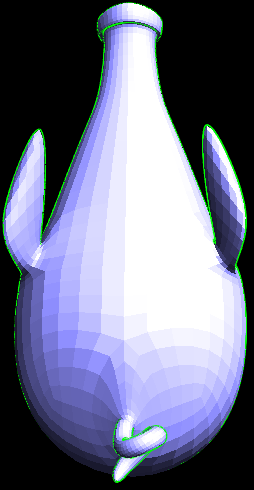
\includegraphics[width=0.25\textwidth]{Pig_patched}
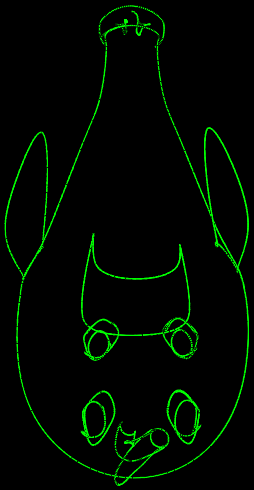
\includegraphics[width=0.25\textwidth]{Pig_silhouettes}
\caption{A view of a pig model and some silhouette curves extracted via our system.}
\label{fig:pig_silhouettes}
\end{figure}


\section{Comparison with prior work}

Past work including \cite{Eisemann08} has extracted silhouette curves from linear patches. They suffer from discontinuity and a lack of accurate interpolation of the points on the surface.
Please see Figure: \ref{fig:Eisemann_linear_patches}. Please see Figure: \ref{fig:torus_silhouette_side_view} for an example silhouette curve that we extracted using our methods that is continuous everywhere and properly follows the surface.


\begin{figure}[h]
\centering
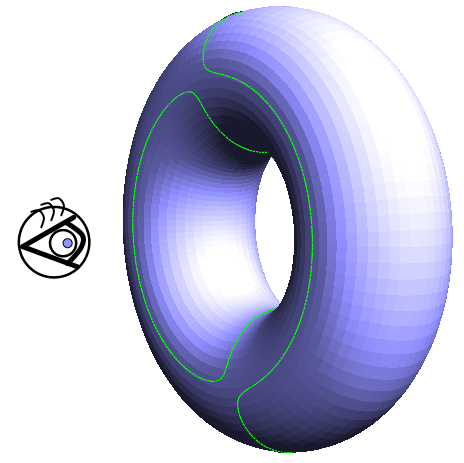
\includegraphics[width=0.5\textwidth]{torus_silhouettes_side_view}
\caption{The curves extracted by our system are continuous even when not viewed by their defining viewing direction.}
\label{fig:torus_silhouette_side_view}
\end{figure}

\newpage

\section{Future Work}

In this discussion, we enumerate several problems that should be addressed in the future,
categorized into those that we feel can be immediatly tackled, those that may need to wait for Mathematics to progress a bit,
and those whose realization is tied to the development of Artifical Intelligence.

	\subsection{Near Term Problems}

	In this section we will describe several coscisely stated problems similar to the silhouette curves problem that may be immediatly tackled in the near future.

		\subsubsection{Extracting the exterior silhouette curve}
		The actual visual exterior for a surface may include subsets of several silhouette curves. The exterior silhouette curve may be computed by projecting the visible

		\subsubsection{Calculation of shadows.}
		We can compute direct shadows	by computing the exterior silhouette curves from a light source viewing in the direction of the surface and then projecting this exterior silhouette 
		onto a plane representing the groud that the surface is resting on.

		\subsubsection{Minnimum and Maximum Curvature Curves}
		Minnimum and maximum curvature curves may be used to communicate information about geometrically intuitive local coordinate systems in the neighborhood of specific points on an object.
		It would be very useful to be able to derive a 2D coordinate grid given a point on a surface.
	
		\subsubsection{Geodesic Curves}
		In the future, a user should be able to specify two points on a surface and receive the curve that represents the minnimum distance path between those two points.
		This is known as the curve of minnimum geodesic distance.
	
		\subsubsection{User Geometric Stylization Scheme}
		My advisor Keenan liked giving presentations with an orange style back in the day, but now he favors blue.
		It would be very useful for users to be able to automatically convert entire presentations, including the images from one style to another.
		A user should be able to define their own figure color scheme in something like a CSS file and be able to automatically convert their figures between styles.

		\subsubsection{Occlusion}

		In our extracted curves, in addition to those points whose normals face away from the camera viewpoint,
		they may also include points that are not visible due to occlusion by other regions of the surface.
		There might be some interesting topological properties of closed curves that could be used for this task,
		especially if the homogenous depth of each of the points from the viewport was taken into account.

	\subsection{Moderate Term Problems}

		In this section, we describe several problems that are more difficult,
		mainly because they involve geometric computations of a higher degree than the current mathematics of our day can handle.
		
		\subsubsection{Perspective Correct Silhouette Curves}
		Right now, we are assuming that the user is viewing the surface with an orthonormal view perspective where the eye is looking in one uniform direction.
		This approximation leads to visually acceptable silhouette curve computations, but it is not accurate in terms of the actual perspective projection that the figures are rendered in.
		To compute the curves in a perspective correct manner would require higher degree geometric computations 

		\subsubsection{Extracting Exact Geometric Curves}
		Right now we are extracting points and tangents along curves, but if people were solve the problem determining the root cuves of multinomials, then we could represent these curves without discretization.

		\subsubsection{Labelling Geometry}

		It would be interesting to develop algorithms for properly placing textual labels for a given figure view where the labels are aware of the geometry.
		The labels placing would have to take into account desirable properties, such as avoiding overlapping lines, avoiding intersections with other labels, and encouraging visual orientation coherence, whereby the labels would all face roughly the same way.
		Arrows could also be investigated.

		\subsubsection{2D Segmenting and Labelling of Ray Traced Imagery}

		A system could hypothetically be built that segments a 2D projection of a ray traced scene into different regions based on light transport phenomena.
		Please see Figure \ref{fig:cornell_box_illustration}.

		\begin{figure}[h]
		\centering
		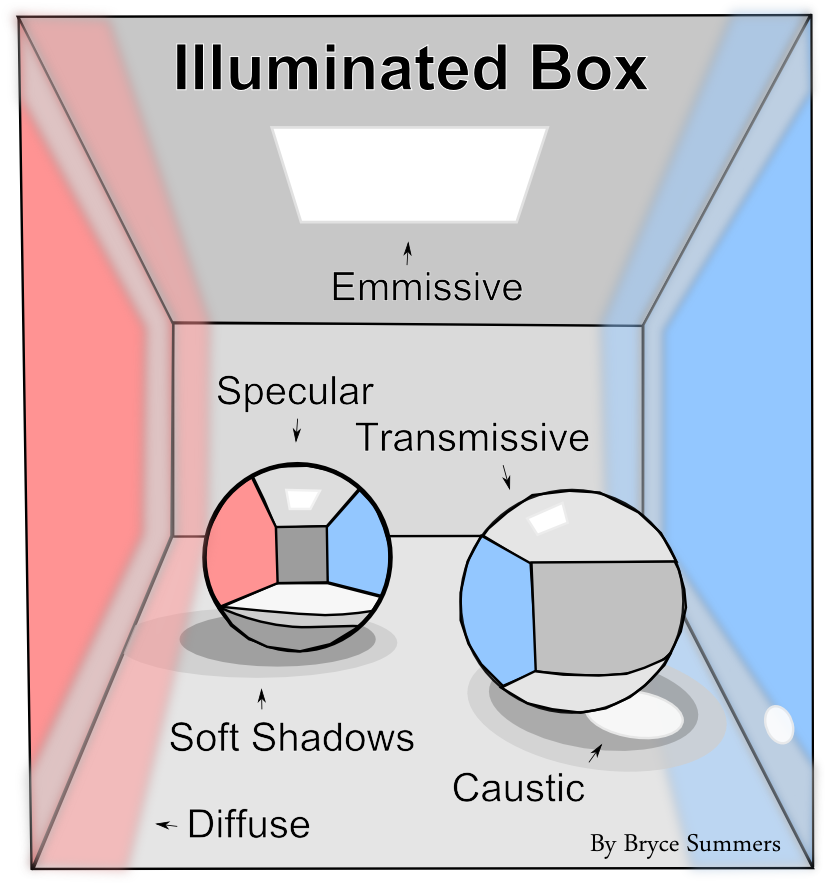
\includegraphics[width=0.5\textwidth]{cornell_box_illustration}
		\caption{A labeled illustration of the idea of converting a ray tracable scene into an SVG file with regions segmented by light transport phenomena.}
		\label{fig:cornell_box_illustration}
		\end{figure}


	\subsection{Long Term Problems}

		In this section, we will describe some long term grand problems that synthesize our work with Artificial Intelligence.

		\subsubsection{Automatic Paper Interpretter}
		In the future, it would be amazing if a user could take a confusing research paper or any other work of communication feed it into a system and get a perfectly clear version of the paper back
		that contains automatically generated illustrations of the ideas contined therin.

\newpage

\section{References}

\begin{thebibliography}{9}

\bibitem{JDA08}
Tilke Judd, Frédo Durand, and Edward Adelson. 2007. 
\emph{Apparent ridges for line drawing}. ACM Trans. Graph. 26, 3, Article 19 (July 2007). DOI=http://dx.doi.org/10.1145/1276377.1276401

Elmar Eisemann, Holger Winnemöller, John C. Hart, and David Salesin. 2008.
\emph{Stylized vector art from 3D models with region support}. In Proceedings of the Nineteenth Eurographics conference on Rendering (EGSR '08). Eurographics Association, Aire-la-Ville, Switzerland, Switzerland, 1199-1207. DOI=http://dx.doi.org/10.1111/j.1467-8659.2008.01258.x

\bibitem{Eisemann08}
Elmar Eisemann, Holger Winnemöller, John C. Hart, and David Salesin. 2008.
\emph{Stylized vector art from 3D models with region support}. In Proceedings of the Nineteenth Eurographics conference on Rendering (EGSR '08). Eurographics Association, Aire-la-Ville, Switzerland, Switzerland, 1199-1207. DOI=http://dx.doi.org/10.1111/j.1467-8659.2008.01258.x

\bibitem{Catmull98}
E. Catmull and J. Clark. 1998. \emph{Recursively generated B-spline surfaces on arbitrary topological meshes.}
In Seminal graphics. ACM, New York, NY, USA 183-188. DOI=http://dx.doi.org/10.1145/280811.280992

\bibitem{Loop}
Charles Loop and Scott Schaefer. 2008.
\emph{Approximating Catmull-Clark subdivision surfaces with bicubic patches}.
ACM Trans. Graph. 27, 1, Article 8 (March 2008), 11 pages. DOI=http://dx.doi.org/10.1145/1330511.1330519

\bibitem{XJY98}
Li Xuejun, Sun Jiaguang, and Yang Changgui. 1998.
\emph{Extracting Silhouette Curves of NURBS Surfaces by Tracing Silhouette Points}.
Tsinghua Science and Technology. ISSN 1007-0214, 13/22, pp1005 - 1008, Volume 3, Number 2. (June 1998), 4 pages.


http://www2.cs.uh.edu/~chengu/Teaching/Spring2013/Lecs/Lec8.pdf

Keenan Crane's Powerpoint presentation about 3D illustration.

\end{thebibliography}

\newpage

		\begin{figure}[h]
		\centering
		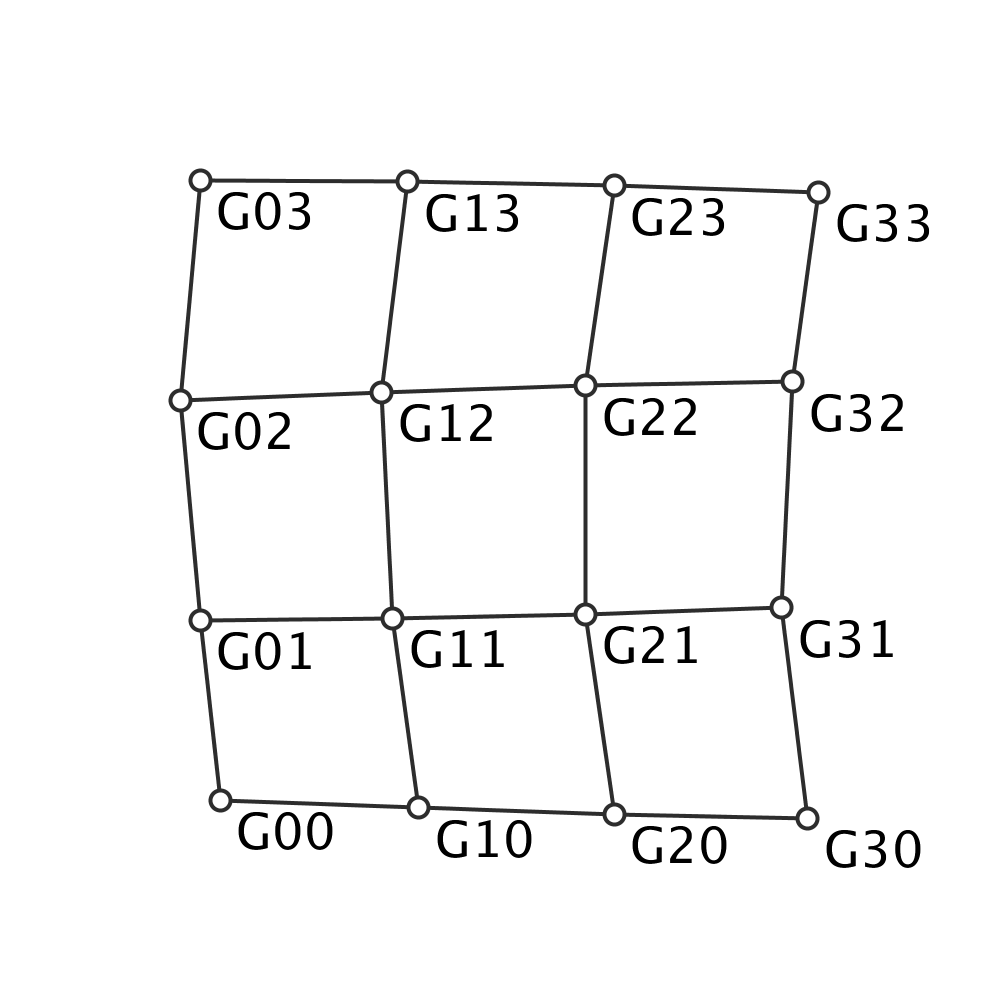
\includegraphics[width=0.5\textwidth]{GeometryPatchControlPoints}
		\caption{Geometry Patch Control Points for a single control mesh face.}
		\label{fig:G}
		\end{figure}
		
		\begin{figure}[h]
		\centering
		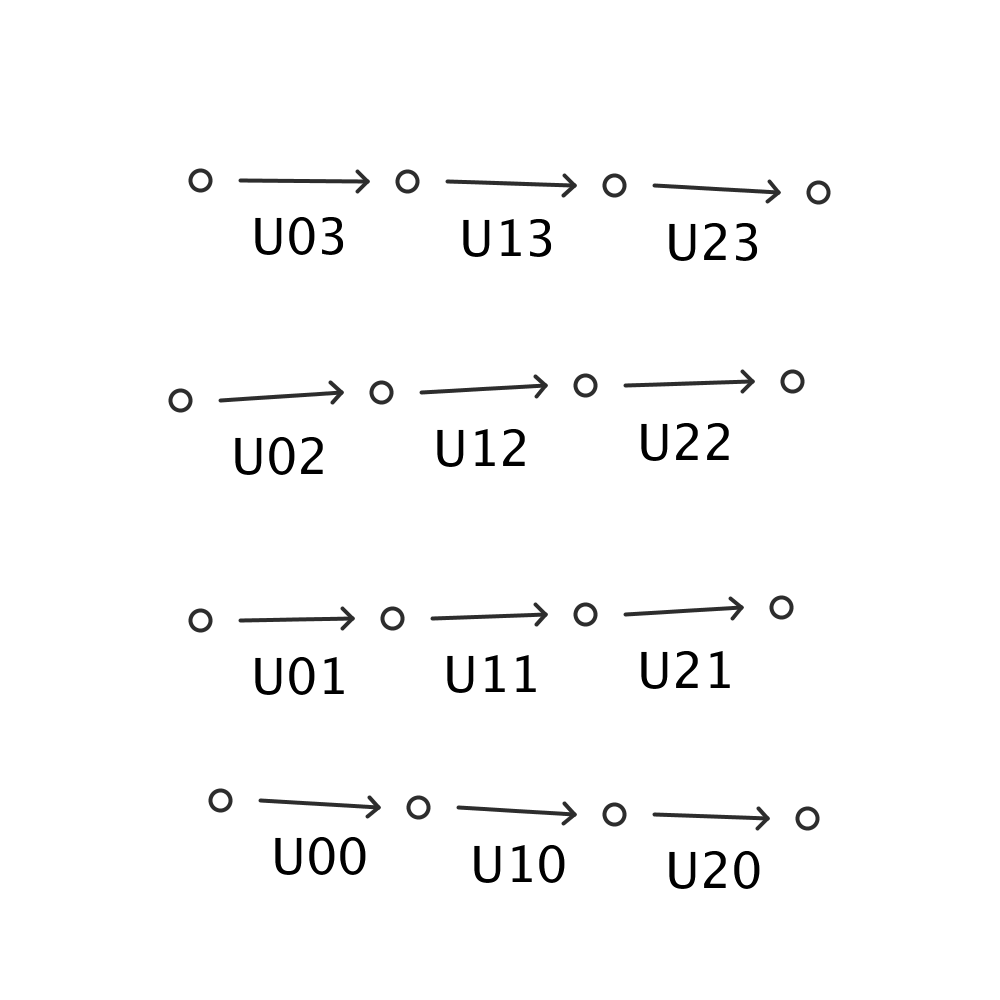
\includegraphics[width=0.5\textwidth]{duPatch}
		\caption{$\partial u$ tangent patch control vectors for a single control mesh face.}
		\label{fig:dU}
		\end{figure}
		
		\begin{figure}[h]
		\centering
		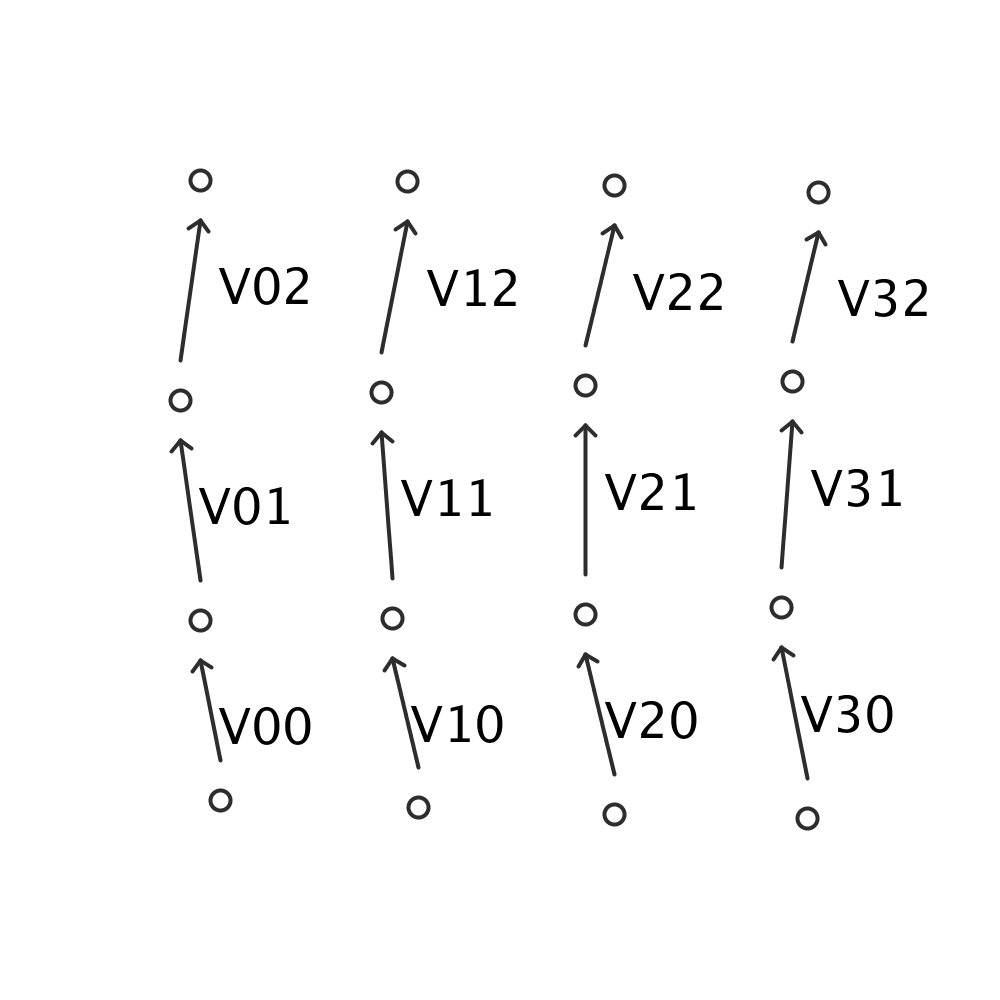
\includegraphics[width=0.5\textwidth]{dvPatch}
		\caption{$\partial v$ tangent patch control vectors for a single control mesh face.}
		\label{fig:dV}
		\end{figure}

\end{document}